% Setup - do not change
\documentclass[11pt]{article}
\usepackage[top=0.9in, left=0.9in, bottom=0.9in, right=0.9in]{geometry}
\usepackage[skip=4pt]{parskip}

\usepackage[english]{babel}
\usepackage[utf8]{inputenc}
\usepackage{amsmath,amsthm,amssymb,graphicx,pdfpages,hyperref}
\usepackage{csquotes}
\usepackage{MnSymbol}

\setlength\parindent{0pt}
%%%%%%%%%%%%%%%%%%%%%%%%%%%%%%%%%%%%%%%%%%%%%%%%%%%%%%%%%%%%%%%%%%%
% add other packages here if required
\usepackage{booktabs}
\usepackage{subcaption}
\usepackage{placeins}
\usepackage{enumitem}
\usepackage{multicol}
\usepackage{graphicx}
\usepackage{wrapfig}
\usepackage{needspace}
\usepackage{titlesec}
\setlist{noitemsep, topsep=2pt, partopsep=0pt}
\setlength{\textfloatsep}{6pt plus 2pt minus 2pt}
\setlength{\intextsep}{4pt plus 2pt minus 2pt}
\setlength{\abovecaptionskip}{3pt}
\setlength{\belowcaptionskip}{1pt}
\setlength{\abovedisplayskip}{6pt plus 2pt minus 2pt}
\setlength{\belowdisplayskip}{6pt plus 2pt minus 2pt}
\setlength{\abovedisplayshortskip}{3pt plus 2pt minus 1pt}
\setlength{\belowdisplayshortskip}{3pt plus 2pt minus 1pt}
\titlespacing*{\section}{0pt}{8pt plus 2pt minus 2pt}{4pt plus 1pt}
\titlespacing*{\subsection}{0pt}{6pt plus 2pt minus 2pt}{2pt plus 1pt}
\titlespacing*{\subsubsection}{0pt}{5pt plus 1pt minus 1pt}{2pt}
\raggedbottom

%% Bibliography are specified in this file. You can also choose inline bib style if you want to. But make sure your citation style is consistent (and proper)
% For more details on citation: https://library.unimelb.edu.au/recite
\usepackage[sorting = none]{biblatex}
\addbibresource{references.bib}

%%%%%%%%%%%%%%%%%%%%%%%%%%%%%%%%%%%%%%%%%%%%%%%%%%%%%%%%%%%%%%%%%%% the '%' symbol denotes comments

% Begin document creation
% DELETE THE \lipsum PLACEHOLDERS WHEN YOU BEGIN
\title{\textbf{Uncaptured Demand For New York City Taxis} \\ }
\author{
Calum Moir \\
Student ID: 1352920 \\
\href{https://github.com/cjboingboing/MAST30034\_Python/tree/215d98d2c2cf03b6b3b0f3818c109e233f9f97c1}{Github repo with commit}
}

\begin{document}
\maketitle

\section{Introduction}
% Link to a 30 min tutorial if you require revision: https://www.overleaf.com/learn/latex/Learn_LaTeX_in_30_minutes

In 2025, New York City's yellow and green taxis combined for 42.6 million trips -- barely a sixth of the roughly 232 million rides Uber and Lyft
carried over the same year~\cite{tlc_trip_data} -- a reversal from a market taxis once held almost outright. This paper investigates
the trends and locations of so-called \textbf{Uncaptured Demand} -- taxi zones not serviced to their theoretical ceiling -- for \textbf{taxi fleet operators
and dispatch planners}: the decision-makers positioned to act on a zone-level reallocation, unlike an individual driver who cannot unilaterally redirect
the fleet. Modelling discovers how much certain factors affect uncaptured demand and simulates configurations of those factors to estimate the resulting
shift in demand.

2025 is used as the modelling year throughout: the most recent complete year of data, chosen over the COVID-distorted 2020--2022 window for a realistic
picture of the market as it stands today, with the same pipeline directly extensible to 2026 as a future exercise once that year's data is released. The
TLC Trip Records dataset~\cite{tlc_trip_data} forms the backbone for the analysis that follows; several other datasets were used to account for confounding variables.


\subsection{Datasets}
The TLC trip records dataset is rich with trip information covering every New York City yellow cab (Manhattan areas),
green taxi (outer boroughs) and HVFHV (high volume for-hire vehicle -- rideshare services such as Uber and Lyft) trip. The dataset also contains a service class
called FHV, which covers luxury courier services such as limousines and private charters; these are considered
a different market to yellow/green cab and rideshare competitors and are therefore not analysed.

To supplement the backbone, various other datasets were gathered to form a better basis for explaining why the gap in
the ride-hailing market is so stark. These datasets include:

\begin{enumerate}
    \item \textbf{National Centers for Environmental Information (NCEI) Hourly Weather Report}~\cite{ncei_lcd} --
    the hourly weather report from various weather stations across the city was used for statistics on local weather conditions.

    \item \textbf{Planned Events in New York City}~\cite{nyc_permitted_events} -- provides additional information on a trip's proximity
    to a planned event. The presence of a major event intrinsically affects the number of ride-hailing trips,
    as a large volume of people travel to the same place at a particular time; events can also
    hinder people's ability to travel due to road closures.
\end{enumerate}

% You can have \section{}, \subsection{}, and \subsubsection{}, \section*{}, \subsection*{}, and \subsubsection*{}


\FloatBarrier
\section{Preprocessing}
\label{sec:preprocessing}
\subsection{TLC Data}

The TLC dataset is vast and messy: many instances contain unrealistic figures that skew inferences. The following validity rules were applied to every trip, regardless of service:

\begin{multicols}{2}
\begin{itemize}
    \item[$\thinstar$] Duration $l_{trip} > 1$ min (no cap)
    \item[$\thinstar$] Distance $d_{trip} \in (0.1, 300)$ mi
    \item[$\thinstar$] Base fare $\geq$ USD\$2.50
    \item[$\thinstar$] Tips/tolls/surcharges $\geq 0$
    \item[$\thinstar$] Categorical fields (vendor, rate code, payment, passengers) in valid TLC ranges
    \item[$\thinstar$] Pickup \emph{and} dropoff are real, mapped zones
    \item[$\thinstar$] Pickup date within the target year
\end{itemize}
\end{multicols}

A trip failing any rule is dropped entirely, not nulled. One exception: a growing, internally-consistent block of trips reports rate code/payment/passenger count as null together, traced to a vendor reporting gap rather than bad data -- kept as ``unknown'' (see \texttt{scripts/tlc\_trips.py}). Duplicate rows from monthly data-release overlaps were also removed. Figure~\ref{fig:pipeline_shapes} traces the resulting shape at each step; taxi's lower retention is driven mainly by sub-minute meter starts and implausible GPS-jump distances, consistent with device glitches rather than genuine short hops. Yellow, green, and rideshare arrive with different raw schemas (rideshare has no passenger-count column at all), so each is filtered on its own fields before harmonising to a common 8-column schema (mode, pickup/dropoff zone, pickup time, distance, duration, cost, tip) and unioning into one trip fact table.

\subsection{Weather data}

The raw hourly weather feed (NCEI LCD pull, LaGuardia station USW00014732) mixes routine hourly METAR reports (report type FM-15) with special reports issued during changing conditions (FM-16) and coarser daily/monthly summary rows (FM-12/SOD/SOM) whose fields are not hourly readings at all. Keeping only FM-15/FM-16 and collapsing to one row per calendar hour -- via a group-by that averages temperature and takes the maximum precipitation across any duplicate reports in the same hour (Figure~\ref{fig:pipeline_shapes}) -- covers 8{,}645 of the year's 8{,}760 hours; the remaining 115 hours have no matching report and stay null after the join, handled the same way as the model's other undefined covariates (missing-indicator method, Section~\ref{sec:feature_design}). Within this filtered set, fields were nulled in one of three ways: categorical blanks (weather/report type) to `Unknown' where no true value could be inferred; blank rain ($32.7\%$ of rows) to zero (no rain); and the sentinel `T' (trace rain) to 0.05mm.

\subsection{Events Data}

NYC's Permitted Events dataset covers millions of permits since 2008, the overwhelming majority (youth/adult sport, farmers markets, sidewalk sales, etc.) too minor to plausibly shift ride-hailing volume. Restricting to 2025 and to \textbf{Parade} and \textbf{Athletic Race/Tour} -- the only categories tied to large-scale street closures capable of measurably affecting trip volume (see \texttt{scripts/generate\_design\_matrix.py}) -- leaves the 587 events used, after dropping one row with an invalid end-before-start timestamp (Figure~\ref{fig:pipeline_shapes} traces each filtering step).

\subsection{Design Matrix Assembly}

Trip, weather, and event summaries are joined onto a scaffold enumerating every (zone, hour) combination that should exist, so an hour with zero trips is an explicit zero, not a missing row. Each subsequent left join preserves this row count while adding columns (Figure~\ref{fig:pipeline_shapes}); the harmonic, lag, and one-hot zone-dummy blocks built on top (Sections~\ref{sec:harmonics} and~\ref{sec:feature_design}) bring the final matrix to the $\sim$290 columns used for modelling (Section~\ref{sec:modelling}).

\begin{figure}[htbp]
\centering
\begin{minipage}[t]{0.48\linewidth}
\fontsize{7.5}{8.3}\selectfont\ttfamily
\begin{verbatim}
YELLOW    load raw trips          (48.7M, --)
          apply validity rules    (42.1M, --)  87%
GREEN     load raw trips          (591K, --)
          apply validity rules    (490K, --)  83%
RIDESHARE load raw trips          (243.6M, --)
          apply validity rules    (~232.2M, --) 95%
ALL       harmonise + union       (274.7M, 8)
WEATHER   load raw hourly feed    (13208, 8)
          keep FM-15 / FM-16      (9991, 8)
          collapse to 1 row/hour  (8645, 4)
\end{verbatim}
\end{minipage}
\hfill
\begin{minipage}[t]{0.48\linewidth}
\fontsize{7.5}{8.3}\selectfont\ttfamily
\begin{verbatim}
EVENTS    load raw permits        (2906868, 13)
          parse timestamps        (2906868, 15)
          keep year = 2025        (278449, 15)
          keep Parade/Athletic    (588, 15)
          drop end < start        (587, 15)
          select needed cols      (587, 5)
DESIGN    zone x hour scaffold    (2303880, 2)
MATRIX    + trip aggregates       (2303880, 16)
          + event counts          (2303880, 17)
          + weather                (2303880, 20)
          + harmonics/lags/zones  (2303880, ~290)
\end{verbatim}
\end{minipage}
\caption{Preprocessing pipeline: transformation steps and the resulting DataFrame shape (rows, columns) at each stage. Percentages are the share of raw rows retained after validity filtering.}
\label{fig:pipeline_shapes}
\end{figure}

\subsection{Engineered Features}

\begin{itemize}
    \item[$\star$] TLC reports no taxi ID, so a na\"ive proxy for zone-level taxi presence, Little's Law's
          \texttt{effective\_taxis = taxi\_trip\_count * avg\_duration}, would be circular as a model feature -- it is computed from the same cell's own trip
          count, the quantity being predicted.
    \item[$\star$] Daily/weekly/yearly harmonic features let the model capture seasonality more naturally than hour-of-day dummies (construction and
          justification in Section~\ref{sec:harmonics}).
\end{itemize}

\FloatBarrier
\section{Analysis and Geospatial Visualisation}
\label{sec:analysis}

To motivate the modelling choices in Section~\ref{sec:modelling}, this section surveys rider patterns across three lenses: the seventeen-year market shift, seasonal/weather effects, and zone-level geography.

NULL handling is detailed in Section~\ref{sec:preprocessing} (weather nulling); Section~\ref{sec:preprocessing}'s validity rules additionally remove 13.5\% of raw yellow/green rows and 4.7\% of raw rideshare rows, concentrated in sub-minute meter starts and implausible GPS-jump distances -- consistent with device/meter glitches rather than genuine short trips being discarded.

\begin{wrapfigure}{r}{0.45\textwidth}
    \centering
    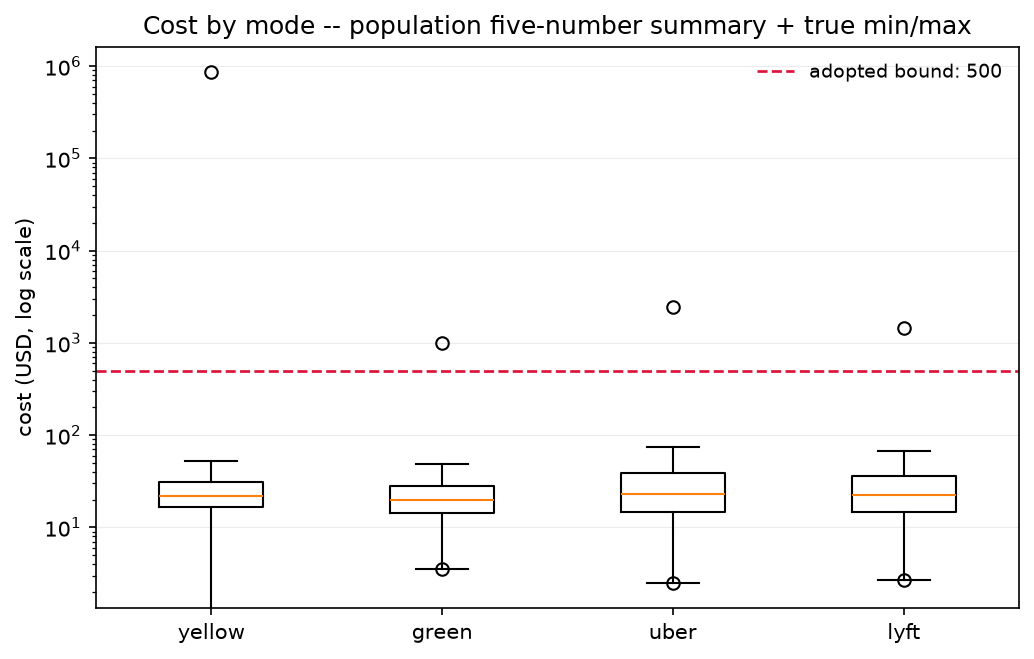
\includegraphics[width=0.98\linewidth]{../plots/outlier_cost_boxplot_2025.png}
    \caption{\label{fig:outlier_cost}Cost by mode (log scale); fliers mark the true population min/max. Dashed line: adopted \$500 bound.}
\end{wrapfigure}

A separate outlier analysis (\texttt{notebooks/general\_stats.ipynb}) examined the full-population distribution (not a subsample) of distance, duration, cost, and tip per mode. Distance was already well-bounded by the existing (0.1, 300)mi rule. Duration and cost were not: yellow taxi's maximum recorded duration was 14{,}880.8 minutes ($\sim$10.3 days) and maximum cost \$863{,}380.37 -- both pass every rule in Section~\ref{sec:preprocessing} unchanged, since neither field previously had an upper bound. The conventional $Q_3 + 1.5\times\text{IQR}$ fence was considered and rejected: for yellow cost it evaluates to \$52.73, which would flag the airport average fare of \$82.6 (Section~\ref{sec:analysis}) as an outlier, and for duration it evaluates to 40.0 minutes against a 40.8-minute JFK-trip average -- the fence catches ordinary long/expensive trips, not just corrupted ones. Bounds were instead set by inspecting the boxplots directly (Figure~\ref{fig:outlier_cost}): duration $\leq 300$ min and cost $\leq$ \$500 (trip dropped), generous enough to keep every plausible real trip while excluding values off by orders of magnitude. Tip, not a model feature, is nulled rather than dropped above \$200. All three are enforced in \texttt{tlc\_trips.py}, upstream of every consumer including the design matrix.

\subsection{Long-Run Context: 2009--2025}

\needspace{6\baselineskip}
\begin{wrapfigure}{l}{0.6\textwidth}
    \centering
    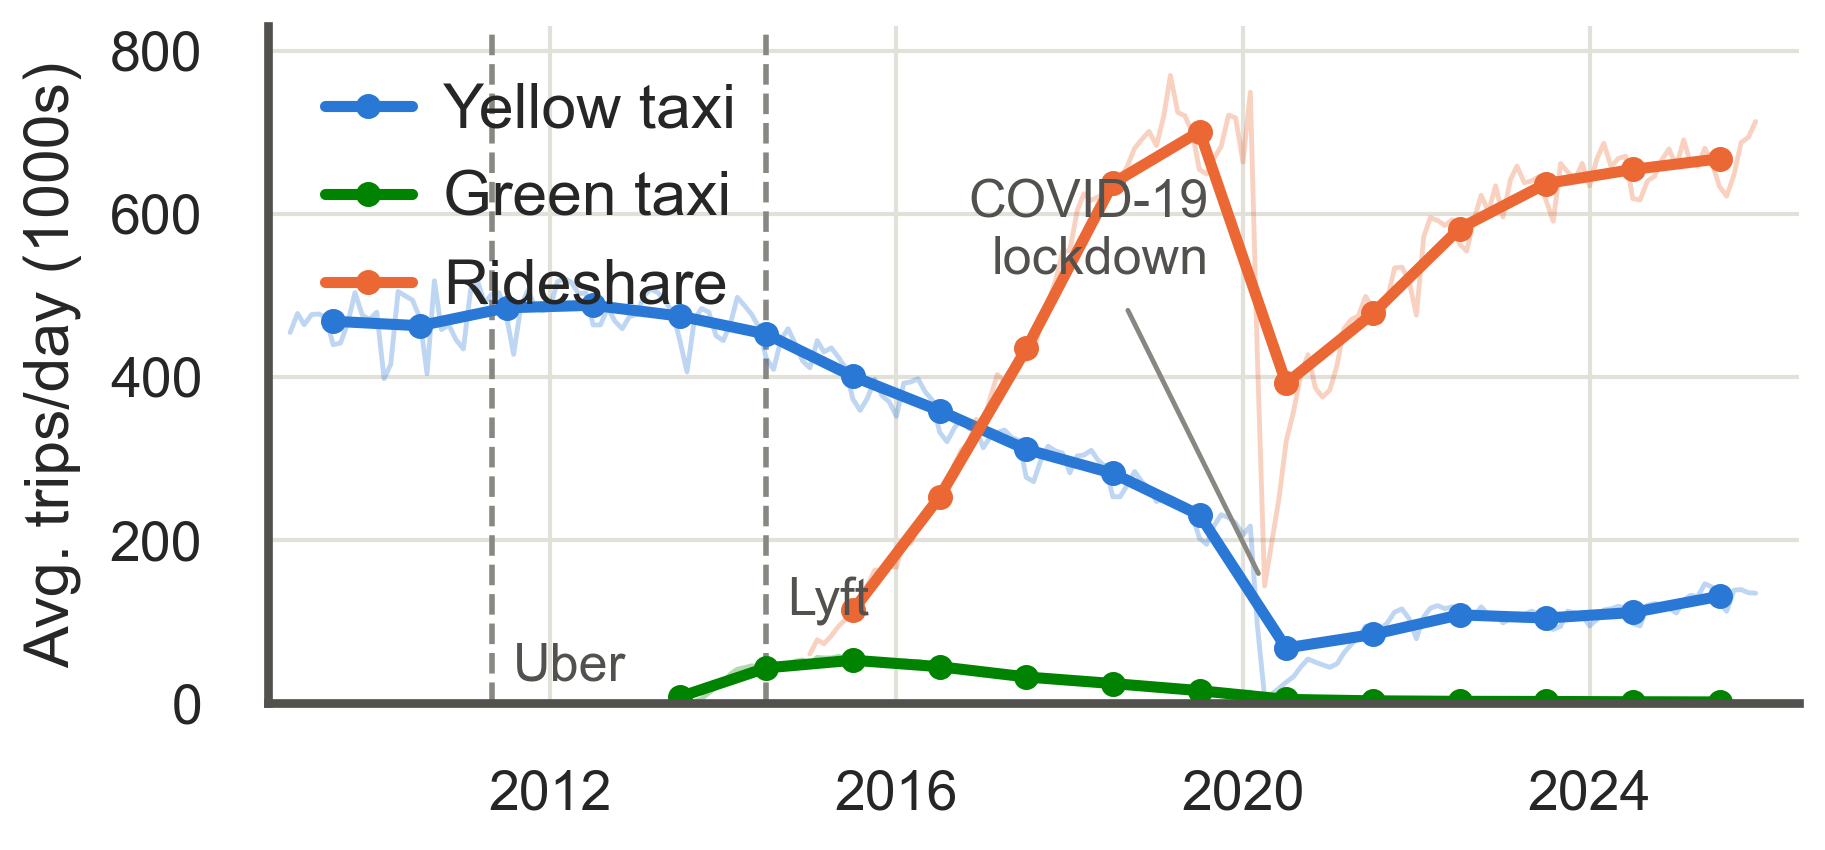
\includegraphics[width=0.98\linewidth]{../plots/longrun_trips_timeseries_2009_2025.png}
    \caption{\label{fig:longrun}NYC taxi vs.\ rideshare trips per day, 2009--2025 (thin: monthly; bold: annual average).}
\end{wrapfigure}


Figure~\ref{fig:longrun} shows the long-run ride-hailing market shift. With a slight lag after rideshare's introduction, both
yellow and green taxi volumes begin to plummet. COVID-19 causes a uniform drop, and yellow cabs appear barely able to recover, while
rideshare sees a steady, unambiguous return to pre-COVID levels.

\needspace{9\baselineskip}
\subsection{Holidays and Seasonality}

\begin{wraptable}{l}{0.48\textwidth}
\centering
\footnotesize
\begin{tabular}{lrr}
\toprule
Holiday & Total (vs.\ wind.) & Taxi (vs.\ wind.) \\
\midrule
Super Bowl LIX (Feb 9)  & 780{,}447 (+3.3\%)   & 14.4\% (14.9\%) \\
Thanksgiving (Nov 27)   & 693{,}714 ($-$7.2\%)  & 9.8\% (13.4\%)  \\
Christmas (Dec 25)      & 564{,}997 ($-$21.5\%) & 11.3\% (13.7\%) \\
New Year's Eve (Dec 31) & 838{,}288 (+28.1\%)   & 11.6\% (12.8\%) \\
\bottomrule
\end{tabular}
\caption{Holiday-day totals vs.\ the surrounding window average. Taxi share falls below its own window average on every holiday.}
\label{tab:holidays}
\end{wraptable}

Across all major holidays, taxis see a decline in trips served per zone while rideshare absorbs the difference -- taxi drivers are
typically full-time employees who take holidays off, whereas rideshare supply is more elastic (Table~\ref{tab:holidays}). New Year's
Eve is the one holiday where total volume rises sharply rather than falling, yet taxi's share still drops below its window average --
evidence that it is rideshare's more elastic supply, not simply lower demand, driving the pattern on every holiday.

\begin{figure}[htbp]
    \centering
    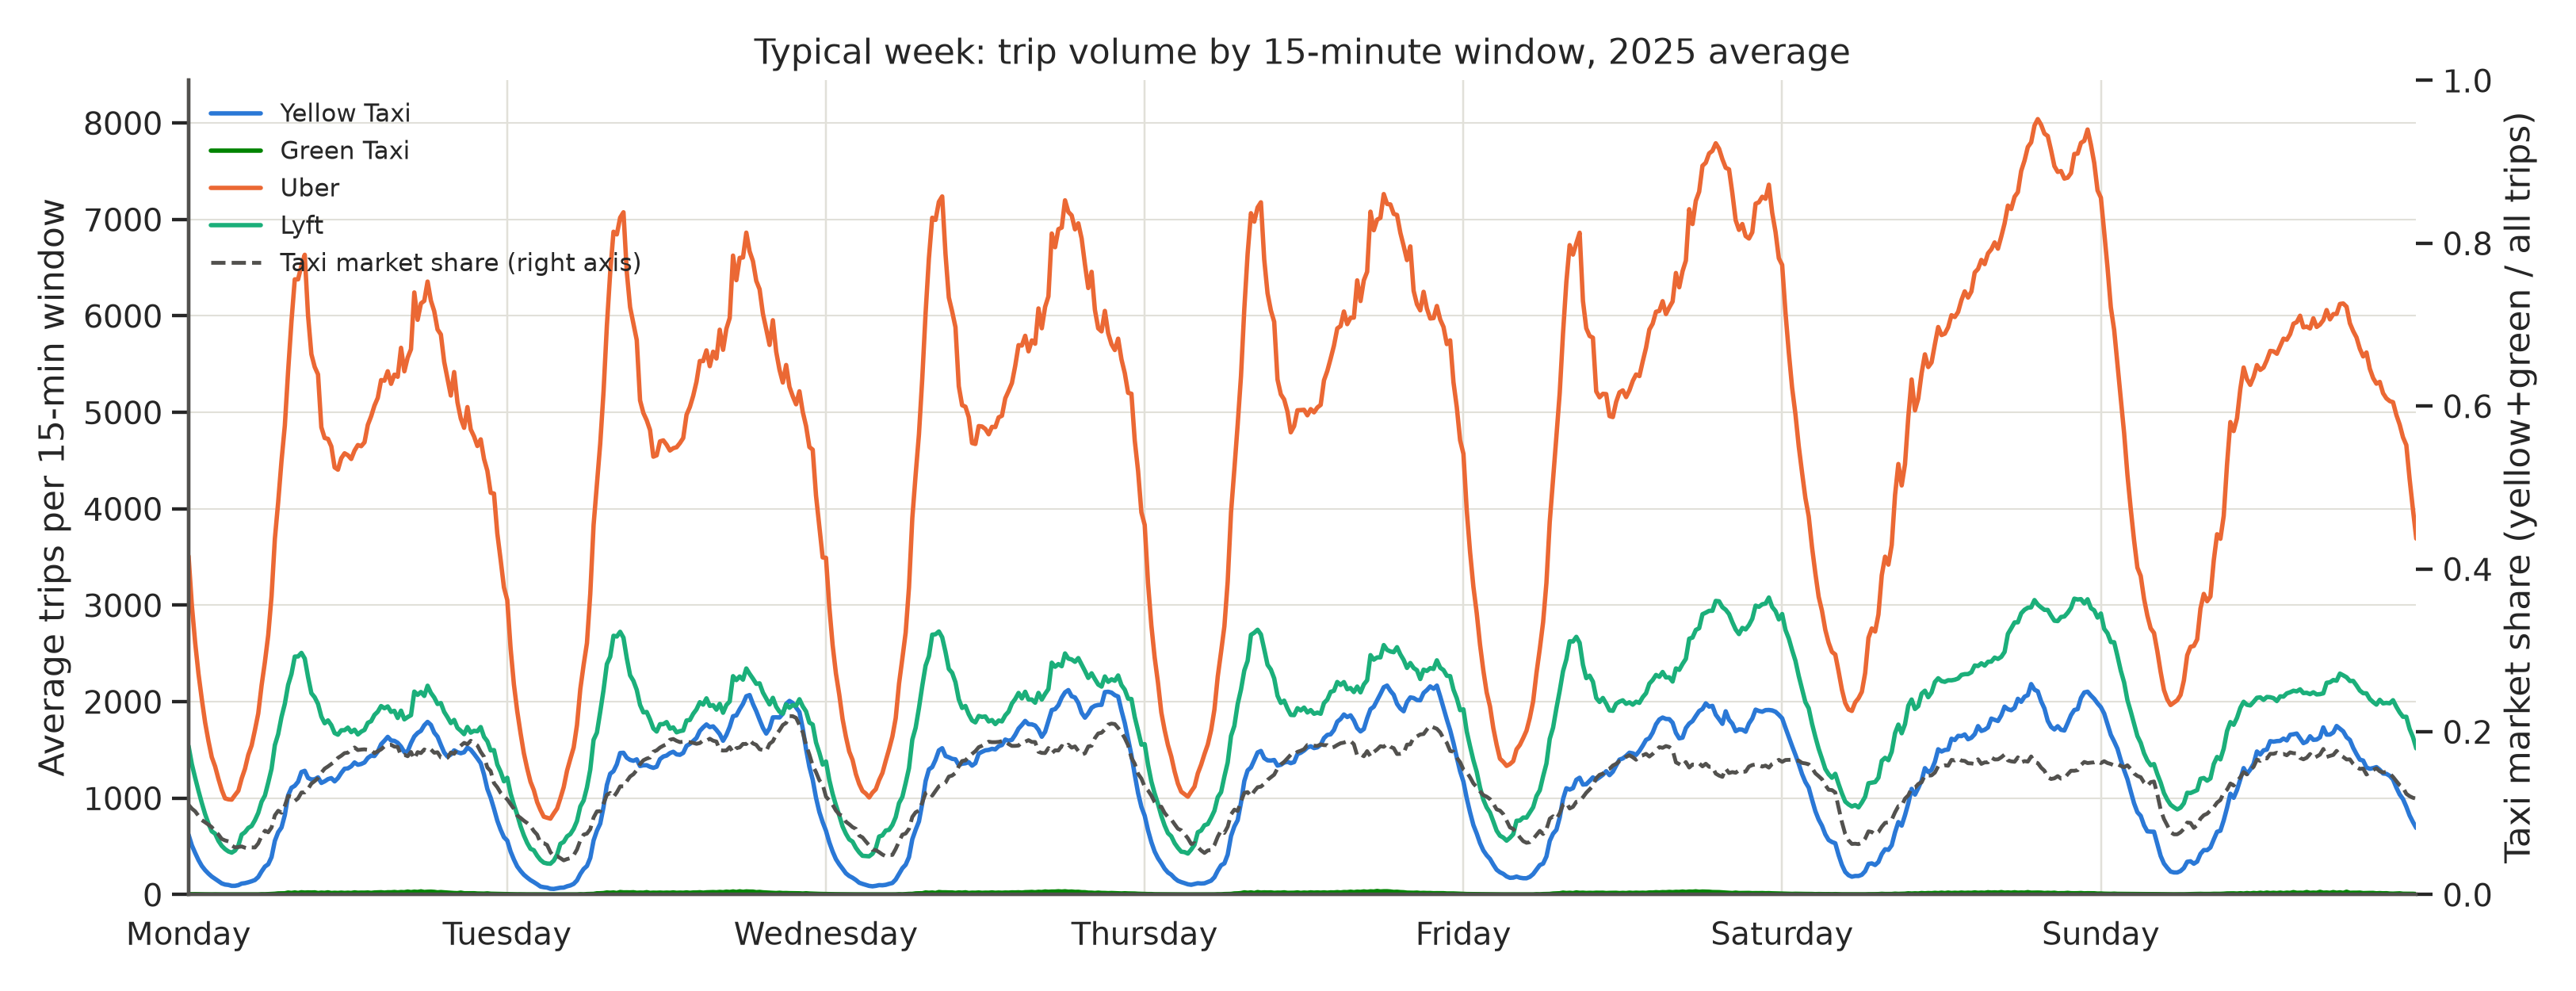
\includegraphics[width=0.85\linewidth]{../plots/typical_week_15min_profile_2025.png}
    \caption{Typical week, 15-minute resolution, 2025 average.}
    \label{fig:typical_week}
\end{figure}

Trip volume swings by almost two orders of magnitude across a typical week (Figure~\ref{fig:typical_week}) -- from a Tuesday
pre-dawn trough (58 avg.\ yellow-taxi trips) to a Saturday-night peak (2{,}182) -- while taxi's own market share moves on a different,
out-of-phase clock, peaking Tuesday evening (21.9\%) and troughing in the Tuesday small hours (4.2\%). Total demand and taxi's
relative competitiveness therefore follow distinct rhythms within the week, motivating the harmonic features of
Section~\ref{sec:harmonics} rather than a single seasonal dummy.

\subsection{Weather Effects}

\begin{table}[htbp]
\centering
\begin{subtable}[t]{0.48\linewidth}
\centering
\footnotesize
\begin{tabular}{lrr}
\toprule
Mode & $r$ (temp) & $r$ (precip) \\
\midrule
Yellow & 0.03  & 0.15$^{**}$  \\
Green  & $-$0.06 & 0.12$^{*}$   \\
Uber   & $-$0.44$^{***}$ & 0.20$^{***}$ \\
Lyft   & $-$0.02 & 0.15$^{**}$  \\
\bottomrule
\end{tabular}
\caption{Pearson $r$, daily. $^{*}p<.05$ $^{**}p<.01$ $^{***}p<.001$.}
\label{tab:weather_r}
\end{subtable}
\hfill
\begin{subtable}[t]{0.48\linewidth}
\centering
\footnotesize
\begin{tabular}{lrrr}
\toprule
Mode & No Rain & Rain & Change \\
\midrule
Yellow & 4{,}762 & 5{,}168 & +8.5\% \\
Green  & 56.0    & 57.3    & +2.4\% \\
Uber   & 18{,}985 & 20{,}270 & +6.8\% \\
Lyft   & 7{,}269  & 7{,}805  & +7.4\% \\
\bottomrule
\end{tabular}
\caption{Avg.\ hourly trips, raining vs.\ not (Jan--Aug 2025).}
\label{tab:rain_effect}
\end{subtable}
\caption{Weather effects by mode. Uber is the only mode with a significant temperature effect (hot days reduce demand); every mode gains from rain, yellow taxi proportionally most.}
\label{tab:weather}
\end{table}

Analysis of different weather scenarios shows Uber is the only mode with a significant temperature effect -- hot days reduce its
demand -- while every mode gains from rain, yellow taxi proportionally most at $+8.5\%$ (Table~\ref{tab:weather_r}, Table~\ref{tab:rain_effect}).

\subsection{Zone-Level Market Share}

\begin{figure}[htbp]
\centering
\begin{subfigure}[t]{0.48\linewidth}
\centering
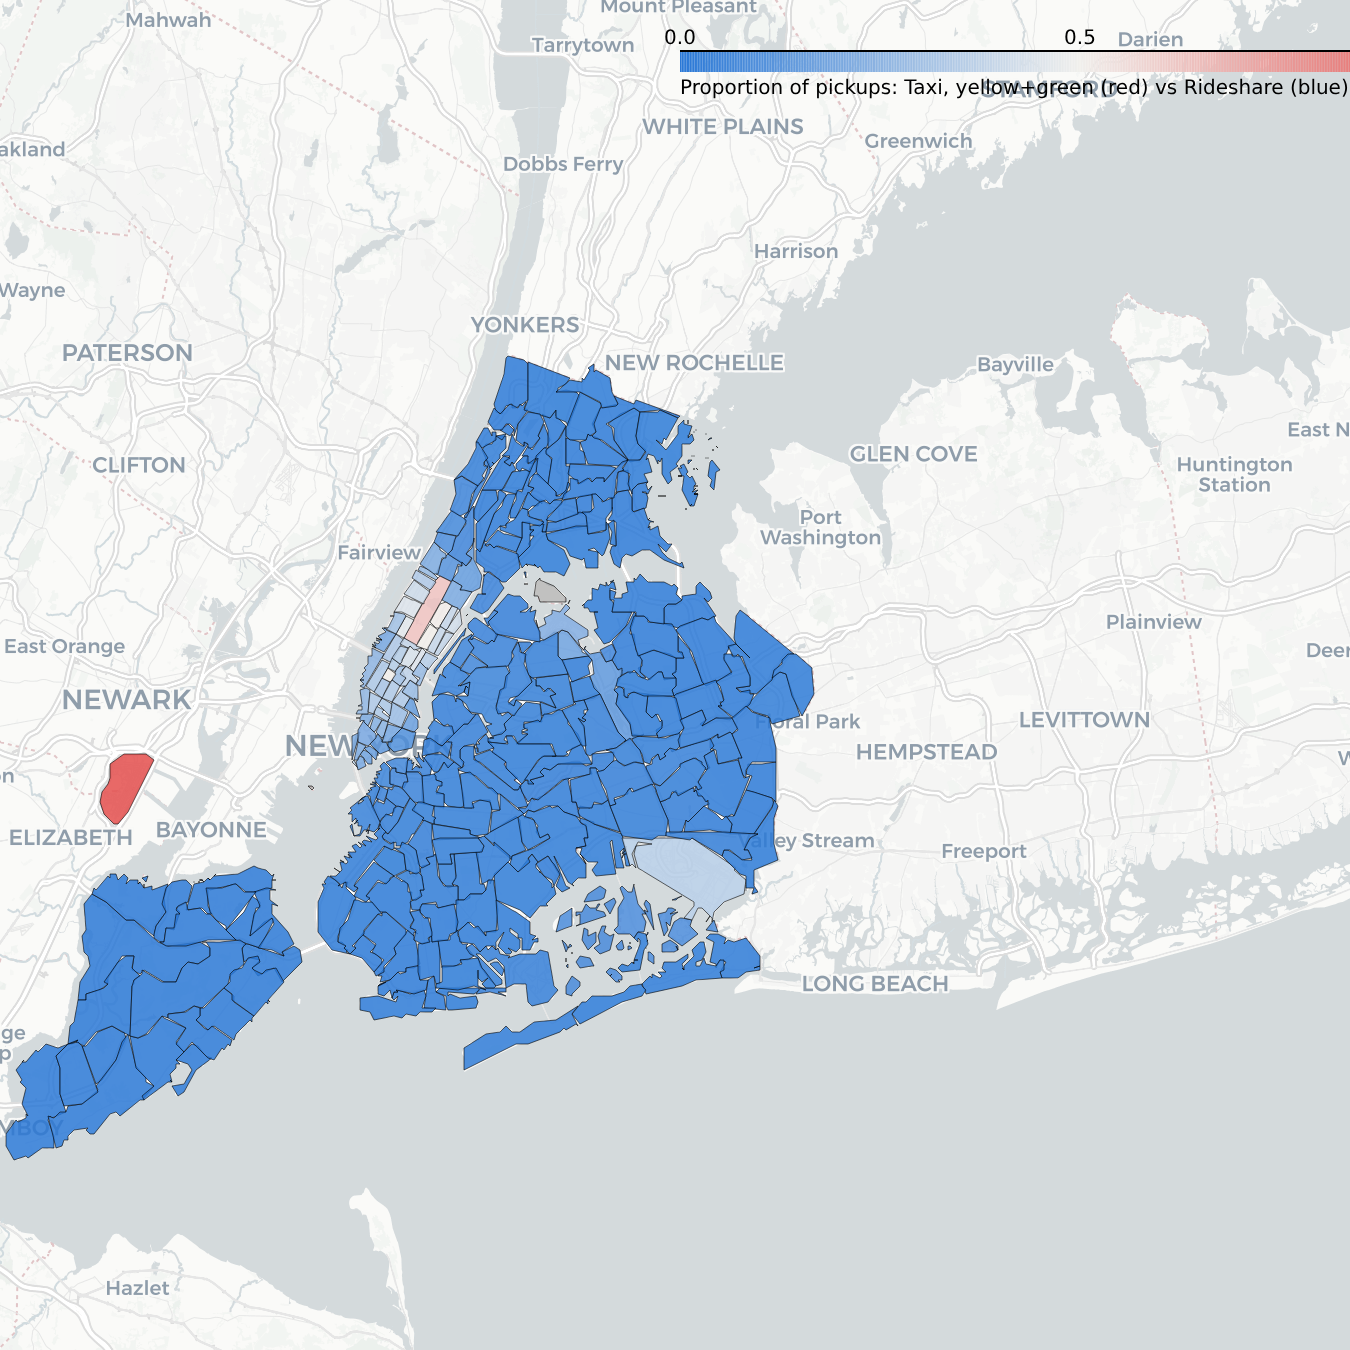
\includegraphics[width=\linewidth]{../plots/screenshots/mode_share_screenshot_crop.png}
\caption{Mode share by zone. \href{https://htmlpreview.github.io/?https://raw.githubusercontent.com/cjboingboing/MAST30034_Python/215d98d2c2cf03b6b3b0f3818c109e233f9f97c1/plots/mode_share_map_2025.html}{Interactive version}.}
\end{subfigure}
\hfill
\begin{subfigure}[t]{0.48\linewidth}
\centering
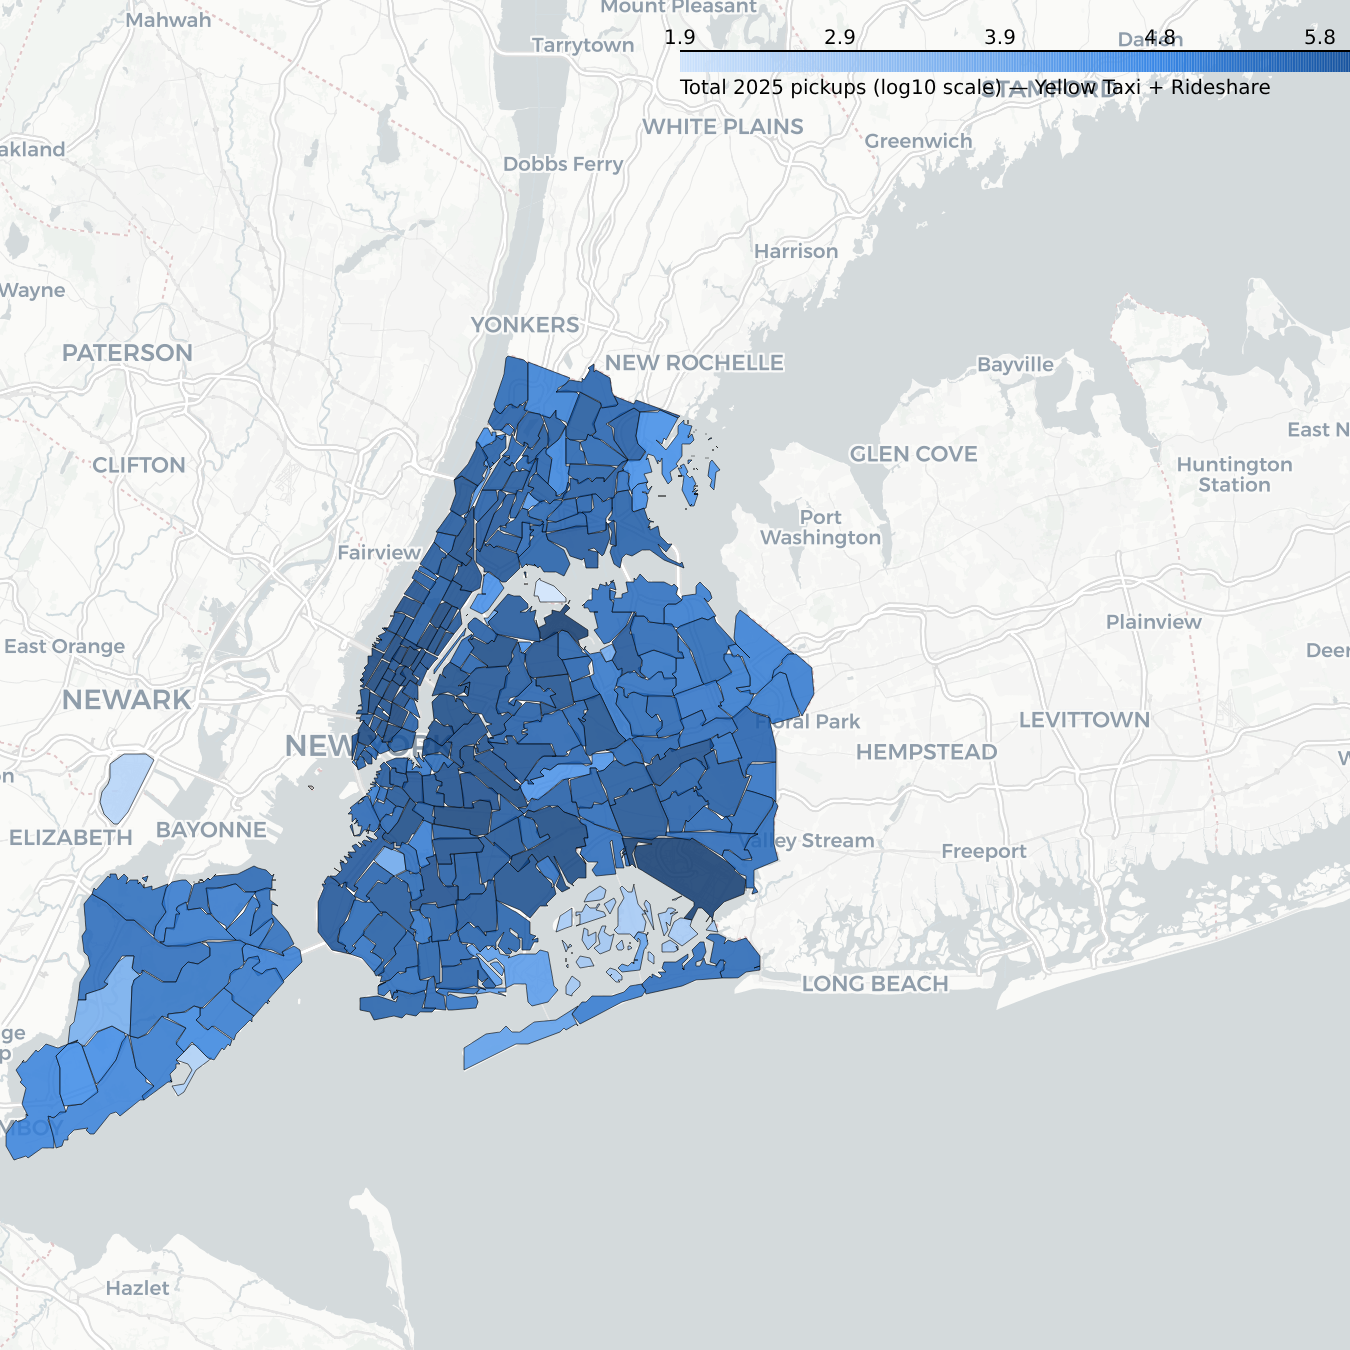
\includegraphics[width=\linewidth]{../plots/screenshots/demand_screenshot_crop.png}
\caption{Total demand by zone, log scale. \href{https://htmlpreview.github.io/?https://raw.githubusercontent.com/cjboingboing/MAST30034_Python/215d98d2c2cf03b6b3b0f3818c109e233f9f97c1/plots/demand_map_2025.html}{Interactive version}.}
\end{subfigure}
\caption{Zone-level taxi/rideshare market share (left) and total 2025 pickup volume (right). Static previews of the interactive choropleths linked above each panel.}
\label{fig:zone_maps}
\end{figure}

At the airports, yellow taxi trips run longer than the cross-service average (JFK: avg.\ 14.1mi/40.8min/\$82.6, +11--20\% dist./dur.\ vs.\ other modes; LaGuardia similar, avg.\ 9.5mi/27.9min/\$66.4) while holding only 6.5--7.4\% of trips at either airport -- Uber alone takes 66--70\%. Green cab's airport share is under 0.2\% at both, too thin to draw conclusions from its otherwise large swings in the underlying data.

Figure~\ref{fig:zone_maps} makes the same split spatial: taxi's demand and share are both concentrated in Manhattan, with Brooklyn/Queens/Bronx zones showing high total volume but near-total rideshare dominance -- consistent with the reallocation analysis in Section~\ref{sec:results}, where several high-\emph{demand} Brooklyn zones sit at just 1--3\% taxi capture, a market effectively already lost rather than merely under-served. This geographic split, not a uniform citywide gap, is why the recommendations in Section~\ref{sec:recommendations} target specific Manhattan zones rather than a blanket fleet expansion.

\FloatBarrier
\section{Modelling}
\label{sec:modelling}

Let $Y_{z,t}$ denote total (taxi $+$ rideshare) trip volume in taxi zone $z$ during hour $t$, and $Y^{taxi}_{z,t}$ the taxi-only component observed internally. All models operate at this (zone, hour) grain -- $263 \times 8{,}760$ cells for 2025.

\subsection{Model Specification}

Observed taxi volume is supply-censored ($Y^{taxi} = \min(\text{demand}, \text{available taxis})$), so total volume is the modelling target -- a cleaner proxy for addressable market. Counts are non-negative and heteroskedastic, so a Poisson GLM with a log link replaces OLS as the starting point, refit Negative Binomial once overdispersion is confirmed (Section~4.5) -- the specification used throughout:
\begin{equation}
    \log \lambda_{z,t} = \mathbf{x}_{z,t}^\top \boldsymbol\beta, \qquad Y_{z,t} \sim \text{Poisson}(\lambda_{z,t}),
\end{equation}
guaranteeing $\lambda > 0$ and a multiplicative rate effect per covariate ($e^{\beta_j}$, an incidence rate ratio).

\subsection{Harmonic (Fourier) Seasonality}
\label{sec:harmonics}

Hour-of-day dummies ignore circularity (hour 23 neighbours hour 0); a sinusoid is the natural basis instead, and the angle-addition identity linearises $A\cos(2\pi t/P-\varphi)$ into ordinary GLM coefficients $a,b$, with $K$ summed harmonics capturing up to $K$ peaks per cycle:
\begin{equation}
    H_P^{(K)}(t) = \sum_{k=1}^{K} \Big[a_k \cos\Big(\tfrac{2\pi k t}{P}\Big) + b_k \sin\Big(\tfrac{2\pi k t}{P}\Big)\Big].
\end{equation}
Three blocks cover demand's natural cycles: $H(t) = H_{24}^{(2)}(t) + H_{168}^{(1)}(t) + H_{8766}^{(1)}(t)$ (daily, weekly, annual). Daily uses $K{=}2$ to separate AM/PM peaks; weekly/annual stay at $K{=}1$ -- one year of data cannot distinguish a higher annual harmonic from a secular trend.

\subsection{Feature Design}
\label{sec:feature_design}

A zone fixed effect $\gamma_z$ pools 263 zones onto shared coefficients, differing only in baseline level. Weather is temperature, precipitation, and a 5-level METAR recode ($\sim$60 raw levels are too sparse individually). Event proximity $x^{ev}_{z,t}$ is chosen empirically from three encodings by held-out deviance. The lag block uses taxi/total counts at $t{-}2,24,168$ (log scale), plus four lag-2 trip-characteristic averages -- undefined, not zero, when no taxi trips occurred -- handled by the missing-indicator method. GLMs are fit on a uniform 5\% subsample, inflating SEs by $\approx 1/\sqrt f$ without biasing point estimates.

\subsection{Full Model Specification}

Stacking weather into $\mathbf{w}_{z,t}$ and lags into $\boldsymbol\ell_{z,t}$:
\begin{equation}
    \log \lambda_{z,t} = \beta_0 + \gamma_z + H(t) + \mathbf{w}_{z,t}^\top \boldsymbol\beta_w + \beta_{ev}\, x^{ev}_{z,t} + \boldsymbol\ell_{z,t}^\top \boldsymbol\beta_\ell,
\end{equation}
261 zone dummies plus the numeric/harmonic/lag blocks give a $\sim$290-column design matrix, purely additive -- every covariate's effect is a constant percentage shift across zones and times -- which the gradient-boosted benchmark below stress-tests.

\subsection{Overdispersion and Robust Inference}

$\text{Var}(Y) = \mathbb{E}[Y]$ is violated ($\hat\phi \gg 1$): unobserved zone-hour heterogeneity (an unflagged event, a driver shortage) pushes some cells past what a single Poisson rate can absorb, inflating variance beyond the mean. The model is therefore refit \textbf{Negative Binomial (NB)}, $\text{Var}(Y) = \lambda + \alpha\lambda^2$ ($\alpha$ via Cameron--Trivedi regression~\cite{cameron_trivedi_count}; nests Poisson at $\alpha=0$) -- the specification used hereafter. Zone-hours also share unmodelled local conditions over time, so inference uses zone-clustered sandwich SEs.

\subsection{Poisson Thinning and Uncaptured Demand}

If each request is served by taxi with probability $p_{z,t}$, the Poisson thinning (colouring) theorem~\cite{ross_probability_models} gives taxi and rideshare counts as Poisson$(\lambda p)$ and Poisson$(\lambda(1-p))$, and the likelihood factorises into the NB count model above and a conditional binomial share, fit separately on the same covariates (excluding lags):
\begin{equation}
    Y^{taxi}_{z,t} \mid Y_{z,t} = n \sim \text{Binomial}(n, p_{z,t}), \qquad \operatorname{logit} p_{z,t} = \mathbf{x}_{z,t}^\top \boldsymbol\theta.
\end{equation}
\textbf{Uncaptured Demand} is $D_{z,t} = \lambda_{z,t}(1-p_{z,t})$, the trips/hour a zone loses to rideshare (ranked in Section~\ref{sec:results}; under NB the two streams are correlated, so $D$ inherits NB's extra dispersion).

\subsection{Benchmark Model}

\texttt{HistGradientBoostingRegressor} (Poisson loss) trains on raw features (untransformed lags, calendar fields, zone target-encoding) as a non-parametric benchmark free to model interactions the additive GLM cannot. Both models plus a seasonal-naive baseline (same hour, last week) are scored on held-out December deviance: GLM for interpretable IRRs, GBM for flexibility.

\FloatBarrier
\section{Results}
\label{sec:results}

The GLM was fit on a uniform 5\% sample of Jan--Nov 2025 (100,887 rows; 261 of 263 zones -- two had zero training-period trips), evaluated against a held-out December 2025 test set (194,184 rows).

\subsection{Model Comparison}

The Poisson fit was strongly overdispersed (Pearson $\hat\phi = 5.98$), so results are reported from its NB refit ($\hat\alpha = 0.0315$). The three event-proximity encodings scored within $0.001$ deviance of each other; the binary indicator was kept as simplest (Table~\ref{tab:model_comparison}).

\subsection{Demand Drivers}

Table~\ref{tab:irr} reports IRRs from the cluster-robust NB fit. Persistence dominates (same hour last week is the strongest predictor), and rain raises demand both as a step and by intensity. Every harmonic term was significant ($p<0.001$); the annual block was only marginal ($p=0.05$), as expected with one year of data.

\begin{table}[htbp]
\centering
\begin{subtable}[t]{0.40\linewidth}
\centering
\footnotesize
\begin{tabular}{lrrr}
\toprule
Model & MAE & RMSE & Dev. \\
\midrule
GBM (trees)     & 20.53 & 42.22 & 6.50  \\
NB GLM          & 23.79 & 50.65 & 9.02  \\
Poisson GLM     & 24.00 & 50.94 & 9.28  \\
Seasonal-naive  & 32.37 & 72.27 & 18.50 \\
\bottomrule
\end{tabular}
\caption{Held-out December 2025 performance. GBM's margin over the NB GLM points to genuine interaction structure (hour$\times$zone$\times$lag) the additive form misses.}
\label{tab:model_comparison}
\end{subtable}
\hfill
\begin{subtable}[t]{0.56\linewidth}
\centering
\footnotesize
\begin{tabular}{lrrr}
\toprule
Term & IRR & 95\% CI & $p$ \\
\midrule
$\log$ demand ($t{-}168$h)  & 1.736 & [1.683, 1.789] & $<0.001$ \\
$\log$ demand ($t{-}24$h)   & 1.269 & [1.246, 1.291] & $<0.001$ \\
$\log$ demand ($t{-}2$h)    & 1.217 & [1.194, 1.240] & $<0.001$ \\
Rain (any)                  & 1.038 & [1.032, 1.045] & $<0.001$ \\
Precip.\ (per mm)           & 1.012 & [1.009, 1.015] & $<0.001$ \\
No taxi, $t{-}2$h           & 1.019 & [1.009, 1.030] & $<0.001$ \\
Nearby event                & 1.010 & [1.003, 1.018] & 0.008 \\
\bottomrule
\end{tabular}
\caption{Selected IRRs, NB GLM, zone-clustered SEs. A no-taxi hour two hours prior predicts \emph{higher} demand -- a supply gap, not a demand lull.}
\label{tab:irr}
\end{subtable}
\caption{Model performance (left) and demand-driver effect sizes (right) from the same NB GLM fit.}
\label{tab:results_pair}
\end{table}

\subsection{Uncaptured Demand by Zone}

The binomial share model (95,525 zone-hours with taxi trips, 253 zones; 8 zero-taxi zones held out at $\hat p = 0$) finds a temperature effect on capture (odds ratio $1.0033$/$^\circ$C, $p<0.001$) but \emph{no} significant weather effect (rain, snow, thunderstorm all $p>0.17$): bad weather raises total demand (Table~\ref{tab:irr}) without shifting the taxi/rideshare split. Combining $\hat\lambda$ and $\hat p$ gives \textbf{Uncaptured Demand}, $D_{z,t} = \hat\lambda_{z,t}(1-\hat p_{z,t})$, ranked in Table~\ref{tab:uncaptured_demand}. A cross-check (swapping observed total for the NB count model's December forecast) gives zone-ranking agreement of Spearman $\rho = 1.000$ across 261 zones -- unaffected by which market-size estimator is used.

\subsection{Revenue Opportunity and Fleet Reallocation}

$D_{z,t}$ translates further: multiplying by the zone's average rideshare fare gives \$827{,}857/hr citywide in fares going to rideshare instead of a yellow cab (same ceiling-not-promise caveat as $D_{z,t}$). Since trip data records no cab count per zone, Little's Law ($L=\lambda W$)~\cite{ross_probability_models} estimates taxis \emph{effectively occupied} by each zone's demand -- a bookkeeping identity needing no queueing assumptions -- implying 1{,}377 taxis in service citywide on average (occupied-with-a-fare only; the true active fleet is larger).

Ranked by uncaptured demand alone, the top zones are almost entirely Brooklyn (Crown Heights North, Bushwick, Williamsburg) -- but these sit at 1--3\% taxi capture, so high uncaptured demand there more likely reflects an unwinnable market than genuine under-supply. Restricting to zones with a real foothold ($\geq10\%$ capture) gives Table~\ref{tab:uncaptured_demand}: LaGuardia, JFK, East Village, Times Sq/Theatre District and Midtown Center are the largest contestable opportunities. Scaling the citywide opportunity by an assumed switchable fraction $s$ gives \$82{,}786/\$165{,}571/\$248{,}357/hr at $s=10/20/30\%$.

\begin{table}[htbp]
\centering
\scriptsize
\begin{tabular}{llrr}
\toprule
Zone & Bor. & Dem./hr & Capt. \\
\midrule
LaGuardia         & QN & 484.1 & 22\% \\
JFK               & QN & 371.5 & 35\% \\
Crown Hts N.      & BK & 357.3 & 2\%  \\
East Village      & MN & 322.9 & 26\% \\
Times Sq/Thea.    & MN & 298.6 & 34\% \\
Midtown Ctr.      & MN & 294.0 & 42\% \\
\bottomrule
\end{tabular}
\caption{Top 6 zones by adjusted uncaptured demand, 2025 avg.\ (full ranking in CSV). Brooklyn pairs high volume with near-total taxi absence; Manhattan shows partial capture; both airports stay majority-uncaptured.}
\label{tab:uncaptured_demand}
\end{table}

\FloatBarrier
\section{Limitations}
\label{sec:limitations}

Several caveats apply across every result and recommendation in this report, stated once here rather
than hedging each number individually:

\begin{itemize}
\item \textbf{Every dollar figure is a hypothetical ceiling, not a promised return.} \$827{,}857/hr
assumes every uncaptured trip converts to a taxi fare -- unrealistic, since some riders are app-native
and unreachable by a street hail regardless of availability. Realistic capture is reported as scenarios
(\$82{,}786/\$165{,}571/\$248{,}357/hr at $10/20/30\%$) rather than a single number, and
Recommendation~\ref{rec:reallocate}'s reallocation estimate should be read the same way.
\item \textbf{This is a prioritisation tool, not a dispatch system.} The NB demand model carries
roughly 17--20\% relative error in Manhattan (Section~\ref{sec:results}) -- enough to rank zone-hours
by opportunity, not to drive minute-by-minute dispatch. Neither model can say \emph{why} a zone
under-performs (price, wait time, habit, local competition).
\item \textbf{No model here observes where cabs currently idle or circulate.} The TLC records contain
no fleet-location data, so \texttt{effective\_taxis} (Little's Law) is a bookkeeping estimate of
fleet-time occupied \emph{with a fare}, not a measured cab count -- and cannot, by construction, say
how capture probability would respond to more cabs being physically sent somewhere.
\end{itemize}

\FloatBarrier
\section{Recommendations}
\label{sec:recommendations}

\begin{enumerate}
\item \label{rec:reallocate} \textbf{Prioritise dispatch/positioning toward LaGuardia, JFK and the
under-served Manhattan zones in Table~\ref{tab:uncaptured_demand}, not Brooklyn.} Ranked by uncaptured
demand alone, the largest gaps are almost entirely Brooklyn (Crown Heights North, Bushwick,
Williamsburg) -- but taxi holds only 1--3\% of trips there against an already-dominant rideshare
market: unwinnable, not under-supplied. Restricting to zones taxi can realistically contest
($\geq10\%$ capture) instead points to the two airports and East Village/Times Square/Midtown Center,
which combine real existing taxi presence with hundreds of uncaptured trips/hour each -- a far more
defensible target list than a blanket citywide expansion.

\item \textbf{Concentrate driver incentives on the specific hours taxi already loses, not general
demand peaks.} Taxi's own share of total demand moves out of phase with demand itself: it peaks at
$21.9\%$ on a Tuesday evening and collapses to $4.2\%$ in the same day's small hours
(Figure~\ref{fig:typical_week}), and falls below its own seasonal-window average on every major holiday
(Table~\ref{tab:holidays}), most sharply at Christmas ($11.3\%$ vs.\ a $13.7\%$ window average) --
exactly when rideshare's more elastic driver supply fills the gap. Shift bonuses timed to these known
low-capture windows are cheaper and faster to deploy than the geographic reallocation above, and can be
trialled alongside it.

\item \textbf{Do not tie dispatch incentives to weather forecasts.} Bad weather reliably grows total
demand -- every mode gains from rain, yellow taxi proportionally most (Table~\ref{tab:rain_effect}) --
but the binomial capture model finds no significant effect of rain, snow or thunderstorm on taxi's
\emph{share} of that demand (all $p>0.17$, Section~\ref{sec:results}); only ambient temperature shifts
the split (odds ratio $1.0033/^\circ$C). A rain-triggered dispatch push would grow a market taxi and
rideshare already share proportionally, not close the gap -- that effort is better spent on
Recommendations 1 and 2, which the data shows actually move the taxi/rideshare split.
\end{enumerate}

\FloatBarrier
\section{Conclusion}

Rideshare did not just grow the ride-hailing market -- it took a large share from taxi, and this paper measures how much of that share is realistically recoverable, and where. \textbf{Uncaptured Demand} decomposes market size from taxi's share of it via Poisson thinning, giving a citywide ceiling of \$827{,}857/hr and a zone ranking honest about its own limits: Brooklyn's largest gaps reflect a market already lost, while Manhattan's partial-capture zones and the airports are worth contesting. The three recommendations act on three levers -- geographic, temporal, and negative (weather moves demand, not the taxi/rideshare split) -- and Section~\ref{sec:limitations} states plainly what none of this claims to be: a prioritisation signal, not a guarantee.


\clearpage

% BEGIN REFERENCES SECTION
\printbibliography

\end{document}